\documentclass[paper=a4,fontsize=12pt,ngerman]{scrartcl}

\usepackage[utf8]{inputenc}				
\usepackage[T1]{fontenc}
\usepackage{graphicx}
\usepackage[ngerman]{babel}
\usepackage{amsmath}
\usepackage[a4paper,left=25mm,right=35mm,top=25mm,bottom=30mm]{geometry}
\usepackage{parskip}
\usepackage{booktabs}
\usepackage{multirow}
\usepackage{float}
\usepackage{amssymb}
\usepackage{csquotes}
\usepackage{url}
\usepackage{listings}
\lstset{
    literate={ä}{{\"a}}1 {ö}{{\"o}}1 {ü}{{\"u}}1 {Ä}{{\"A}}1 {Ö}{{\"O}}1 {Ü}{{\"U}}1 {ß}{{\ss}}1
}
\usepackage{xcolor}
\usepackage{microtype}
\usepackage[hidelinks]{hyperref}
\begin{document}

\pagenumbering{roman}
\pagestyle{plain}

% Einbinden der Titelseite
\begin{titlepage}

\linespread{1.5}


\includegraphics[width=\linewidth]{graphics/htw_logo}

\begin{center}
    \large  
    \hfill
    \vfill
    \Large{\bfseries{Eine historische Betrachtung des Quicksort-Algorithmus}}
    
    von \\
    Klaus Müller

    \vfill
		
    Ein wissenschaftlicher Bericht im Rahmen der Vorlesung\\
    \glqq Wissenschaftliches Arbeiten\grqq\\
    an der htw saar im Studiengang Informatik\\
	
    \vfill	
    \vfill
	
    Saarbrücken, den 17.07.2020
\end{center}
    
\end{titlepage}


% Hier ist der Abstract
\section*{Abstract}
Diese Arbeit untersucht die Architektur und die Anwendungsbereiche von Delay Tolerant Networks (DTN).
Sie richtet sich an Umgebungen, in denen traditionelle Internet-Protokolle aufgrund von langen Verzögerungen und häufigen Verbindungsabbrüchen versagen.
Zunächst werden die grundlegenden Konzepte wie das Store-and-Forward-Prinzip und die Bundle-Protokoll-Architektur vorgestellt.
Anschließend werden die zentralen Anwendungsfelder von DTN, von der Weltraumkommunikation bis zu terrestrischen Notfallnetzen, beleuchtet.
In einer Analyse werden die Vor- und Nachteile von DTN gegenüber traditionellen TCP/IP-Netzwerken herausgearbeitet und die Leistung anhand von Latenz und Datendurchsatz bewertet.
Abschließend werden die Ergebnisse zusammengefasst und ein Ausblick auf zukünftige Forschungsrichtungen im Bereich DTN gegeben.

\newpage
\section*{Selbstständigkeitserklärung}
Ich versichere, dass ich die vorliegende Arbeit selbstständig verfasst und 
keine anderen als die angegebenen Quellen und Hilfsmittel benutzt habe.
Insbesondere habe ich alle KI-basierten Werkzeuge angegeben, die ich bei
der Erstellung, Übersetzung oder Überarbeitung des Textes verwendet habe.

Ich erkläre hiermit weiterhin, dass die vorgelegte Arbeit zuvor weder von mir 
noch von einer anderen Person an dieser oder einer anderen Hochschule 
eingereicht wurde.

Darüber hinaus ist mir bekannt, dass die Unrichtigkeit dieser Erklärung eine 
Benotung der Arbeit mit der Note \glqq nicht ausreichend\grqq \ zur Folge hat 
und einen Ausschluss von der Erbringung weiterer Prüfungsleistungen zur Folge 
haben kann.
\bigskip
 
Saarbrücken, den 30.08.2025

\smallskip





% Das Inhaltsverzeichnis
\clearpage
\tableofcontents 

\clearpage
\pagenumbering{arabic}

% Hier beginnt das erste Kapitel
\section{Einleitung}

\subsection{Motivation: Warum Delay Tolerant Networking?}
Delay Tolerant Networks (DTN) wurden entwickelt, um Kommunikation in Umgebungen zu ermöglichen, in denen traditionelle Netzwerkprotokolle versagen. 
Wie Scott und Burleigh in RFC 5050 definieren: \enquote{Delay Tolerant Networking is an end-to-end architecture providing communications in and/or through highly stressed environments. Stressed networking environments include those with intermittent connectivity, large and/or variable delays, and high bit error rates} \cite[S. 3]{ScBu07}.
Die Weltraumkommunikation motivierte die ursprüngliche Entwicklung, da Signale zwischen Raumsonden und der Erde aufgrund großer Entfernungen mehrere Minuten bis Stunden benötigen.

\subsection{Abgrenzung zum traditionellen Internet}
Kevin Fall beschreibt die grundlegenden Annahmen des traditionellen Internet-Protokolls: \enquote{Although often not explicitly stated, a number of key assumptions are made regarding the overall performance characteristics of the underlying links in order to achieve this service: an end-to-end path exists between a data source and its peer(s), the maximum round-trip time between any node pairs in the network is not excessive, and the end-to-end packet drop probability is small} \cite[S. 27]{Fall03}.
DTN hingegen implementiert ein nachrichtenorientiertes Overlay-Protokoll, das diese Annahmen nicht macht\cite[S. 5]{NASA25}.

\subsection{Zielsetzung der Arbeit}
Diese Arbeit gibt einen Überblick über die grundlegenden Konzepte von DTN, seine Anwendungsbereiche und die damit verbundenen Herausforderungen.
Es werden technische Details erklärt, um ein umfassendes Verständnis dieser Netzwerktechnologie zu vermitteln.


\section{Grundlagen und Funktionsweise von Delay-Tolerant Networking}

\subsection{Store-and-Forward-Nachrichtenvermittlungsprinzip}

Das Store-and-Forward-Prinzip ist ein zentrales Konzept in Delay-Tolerant Networks (DTN), um in Umgebungen mit unterbrochener Konnektivität und langen Verzögerungen zu kommunizieren. 
Dabei speichern Zwischenknoten ganze Nachrichten, die sogenannten Bundles, oder deren Fragmente persistent. 
Der Knoten hält die Daten, bis eine geeignete Verbindung zum nächsten Knoten oder zum Ziel verfügbar ist. 

Dies unterscheidet sich grundlegend von der Paketvermittlung im Internet.
Dort werden Daten nur kurzzeitig in Puffern gespeichert. 
Zusätzlich müssen End-to-End-Pfade kontinuierlich verbunden sein \cite[S. 11]{Wart15}.

\subsection{Bundle-Architektur und Protokolle}

\begin{figure}[H]
\centering
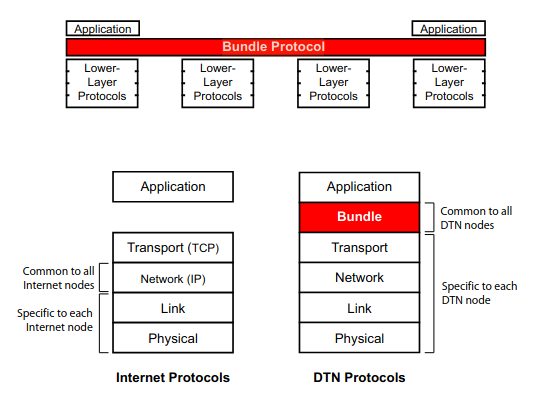
\includegraphics[width=0.7\textwidth]{graphics/BundleProtokol.png}
\caption{Bundle-Protokoll-Architektur als Overlay-Netzwerk \cite[S.15]{Wart15}}
\label{fig:bundleprotokoll}
\end{figure}

Die Architektur von Delay-Tolerant Networks basiert auf dem Bundle Protocol (BP). 
Das BP dient als Overlay-Protokoll und verbindet heterogene Netzwerkinfrastrukturen zu einem interoperablen Gesamtsystem (siehe Abbildung \ref{fig:bundleprotokoll}). 
Es abstrahiert die spezifischen Eigenschaften der darunterliegenden Transportschichten. 
Gleichzeitig schafft es eine einheitliche Schnittstelle für Anwendungen, die auf dem Store-and-Forward-Prinzip aufbaut \cite[S. 6]{CBH+07}.

\subsubsection{Protokollstruktur und Adressierung}

Die fundamentale Dateneinheit im Bundle Protocol ist das \textit{Bundle}. 
Jedes Bundle besteht aus einem \textbf{Primärblock}, der Metadaten wie Quell- und Zieladresse, Erstellungszeitpunkt und Lebensdauer enthält. 
Ein optionaler \textbf{Nutzdatenblock} (Payload) sowie weitere \textbf{Erweiterungsblöcke} ergänzen diesen. 
Diese modulare Struktur ermöglicht die Integration zusätzlicher Funktionalitäten, beispielsweise für Sicherheit (Bundle Security Protocol) oder Quality-of-Service \cite[S. 11-12]{ScBu07}.

Zur Adressierung verwendet man Endpoint Identifiers (EIDs), die als Uniform Resource Identifiers (URIs) strukturiert sind. 
Dieses flexible Schema erlaubt eine von der Topologie unabhängige Benennung von Endpunkten. 
Es unterstützt das Konzept des \textit{Late Binding}, bei dem die Zuordnung eines EIDs zu einer konkreten Netzwerkadresse erst während des Transports erfolgt \cite[S. 7-9]{CBH+07}.

\subsubsection{Convergence Layer und Protokollintegration}

Die Anpassung des Bundle Protocols an unterschiedliche Transporttechnologien erfolgt durch sogenannte \textbf{Convergence Layer Adapter} (CLA). 
Diese Schicht überbrückt die Systemgrenzen zwischen dem Bundle-Layer und den spezifischen Protokollen der unteren Schichten. 
Für stabile Netzwerke kommt oft ein TCP-basierter CLA (TCPCL) zum Einsatz. 
In hochgradig gestörten Umgebungen wie der Weltraumkommunikation bevorzugt man spezialisierte Protokolle wie das Licklider Transmission Protocol (LTP), das für Verbindungen mit hoher Latenz und Asymmetrie optimiert ist \cite [S. 3]{WaWa25}.

\subsubsection{Zuverlässigkeit und Ressourcenmanagement}

Ein zentraler Mechanismus zur Sicherstellung der Zuverlässigkeit ist der \textbf{Custody Transfer}. 
Hierbei übernimmt ein Zwischenknoten (der \textit{Custodian}, dt. Verwahrer) explizit die Verantwortung für die sichere Weiterleitung eines Bundles. 
Das Bundle wird erst nach erfolgreicher Übergabe an den nächsten Custodian auf dem vorherigen Knoten gelöscht. 
Dieser Hop-by-Hop-Ansatz erhöht die Zustellwahrscheinlichkeit in verlustbehafteten Netzwerken signifikant im Vergleich zu reinen End-to-End-Mechanismen \cite{CBH+07}.

Ein zentraler Aspekt bei der Modellierung von DTN-Knoten ist die zeitabhängige Kapazität und Verzögerung. 
Für einen Knoten mit Kapazität $C(t)$ und Verzögerung $D(t)$ zum Zeitpunkt $t$ gilt: Werden $B$ Bits zu diesem Zeitpunkt auf den Knoten gesetzt, erreichen sie den Zielpunkt vollständig zum Zeitpunkt \cite[S. 16]{CBH+07}:

\begin{equation}
t_{\text{arrival}} = t + D(t) + \frac{B}{C(t)}
\end{equation}

Dabei wird unterstellt, dass sich $C(t)$ und $D(t)$ während des Übertragungsintervalls nicht wesentlich ändern.
\newpage
\section{Anwendungsbereiche}

DTN (Delay Tolerant Networks) finden Anwendung in verschiedenen Bereichen, in denen herkömmliche Internet-Protokolle an ihre Grenzen stoßen. 
Tabelle \ref{tab:applications} gibt einen Überblick über die Hauptanwendungsbereiche und deren charakteristische Eigenschaften.

\begin{table}[H]
\centering
\begin{tabular}{|p{4.5cm}|p{5.5cm}|p{5.5cm}|}
\hline
\textbf{Anwendungsbereich} & \textbf{Charakteristika} & \textbf{Beispiele} \\
\hline
Weltraumkommunikation & Hohe Latenz (Minuten bis Stunden), periodische Unterbrechungen & Mars-Rover, Internationale Raumstation, Interplanetare Sonden \\
\hline
Militärische Netzwerke & Intermittierende Konnektivität, Jamming, hohe Mobilität & Battlefield-Kommunikation, Drohnen-Netzwerke, Truppenkoordination \\
\hline
Sensornetzwerke & Begrenzte Energie, geplante Konnektivität, große Knotenzahl & Umweltmonitoring, Smart Cities, Industrielle IoT \\
\hline
Katastrophengebiete & Zerstörte Infrastruktur, Ad-hoc-Verbindungen & Notfallkommunikation, Rettungseinsätze, Koordination \\
\hline
Abgelegene Gebiete & Fehlende Infrastruktur, sporadische Verbindungen & Ländliche Datennetzwerke, Bus-basierte Datenübertragung \\
\hline
Unterwasser-Netze & Akustische Kommunikation, niedrige Datenraten & Meeresforschung, Unterwasser-Roboter, Umweltüberwachung \\
\hline
\end{tabular}
\caption{Hauptanwendungsbereiche von Delay Tolerant Networks \cite[S. 5]{Wart15}, \cite[S. 9--16]{GYL+15}}
\label{tab:applications}
\end{table}

\subsection{Weltraumkommunikation}

Die Weltraumkommunikation war der ursprüngliche Treiber für die DTN-Entwicklung.
Sie stellt bis heute ein wichtiges Anwendungsgebiet dar. Die NASA setzt DTN für verschiedene Missionen ein, darunter die Internationale Raumstation und interplanetare Sonden \cite{NASA25}.
Die extremen Distanzen und die daraus resultierenden Signalverzögerungen erschweren den Einsatz herkömmlicher Protokolle erheblich.

Die Satellitenkommunikation profitiert von den Store-and-Forward-Fähigkeiten von DTN. Diese ermöglichen die Datenübertragung auch bei unterbrochenen Verbindungen.
Erdbeobachtungssatelliten können große Datenmengen sammeln und übertragen, auch wenn direkte Verbindungen zur Erde nur zeitweise verfügbar sind. Relay-Satelliten fungieren als Zwischenspeicher und leiten die Daten weiter, sobald sich eine günstige Verbindung ergibt.

\subsection{Terrestrische Anwendungen}

Neben der Weltraumkommunikation findet DTN in verschiedenen terrestrischen Bereichen Verwendung. Militärische Ad-hoc-Netzwerke profitieren von der Fähigkeit, auch bei gestörten oder unterbrochenen Verbindungen zu funktionieren.
Sensornetzwerke nutzen DTN für die Datenübertragung bei begrenzten Energieressourcen.
In Katastrophengebieten ermöglicht DTN die Kommunikation trotz zerstörter Infrastruktur.

Das Protokoll unterstützt auch die Datenübertragung in abgelegenen Gebieten, wo keine kontinuierliche Netzwerkanbindung verfügbar ist. 
Fall betont hierzu: \enquote{The highly successful architecture and protocols of today's Internet may operate poorly in environments characterized by very long delay paths and frequent network partitions} \cite [S. 1]{Fall03}.

\section{Herausforderungen und Einschränkungen}
\begin{table}[H]
\centering
\begin{tabular}{|p{4cm}|p{5.5cm}|p{5.5cm}|}
\hline
\textbf{Kriterium} & \textbf{Delay Tolerant Networking (DTN)} & \textbf{Traditionelles Netzwerk (TCP/IP)} \\
\hline
Konnektivitäts-Anforderung & Tolerant gegenüber langen Unterbrechungen und hohen Latenzen (Store-and-Forward) & Benötigt eine kontinuierliche End-to-End-Verbindung mit geringer Latenz \\
\hline
Fehlerbehandlung & Robust durch Hop-by-Hop-Bestätigungen (Custody Transfer) & Anfällig bei Paketverlust; verlässt sich auf End-to-End-Retransmission \\
\hline
Speicherbedarf & Hoch; benötigt persistenten Speicher auf Zwischenknoten & Gering; benötigt nur flüchtige Puffer für die Weiterleitung \\
\hline
Komplexität & Hoch; zusätzliche Protokollschicht (Bundle Protocol) als Overlay & Geringer; etablierter und weit verbreiteter Standard \\
\hline
Overhead & Potenziell höher durch Bundle-Header und Metadaten & Optimiert und in der Regel geringer \\
\hline
Interoperabilität & Sehr hoch; kann heterogene Netzwerke (z.B. Weltraum und terrestrisch) verbinden & Begrenzt auf IP-basierte Netzwerke \\
\hline
\end{tabular}
\caption{Vergleich von DTN mit traditionellen Netzwerkarchitekturen \cite{CBH+07,Fall03}}
\label{tab:dtn_vs_tcpip}
\end{table}


\subsection{Latenz und Ressourcenverbrauch}
\begin{figure}[h!]
\centering
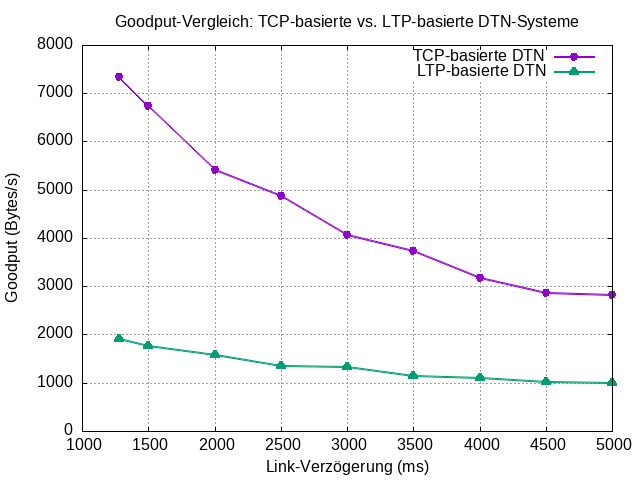
\includegraphics[width=0.8\textwidth]{graphics/dtn_goodput.png}
\caption{Goodput-Leistung verschiedener DTN-Implementierungen in Abhängigkeit von der Link-Verzögerung \cite[S. 5-6]{WaWa25}.}
\label{fig:dtn_goodput}
\end{figure}

Latenz und Ressourcenverbrauch bestimmen die Leistungscharakteristik von DTN-Systemen. Diese Parameter variieren je nach Implementierung und Anwendungskontext. DTN-Implementierungen operieren mit extremen Verzögerungen von Minuten bis Tagen und stellen besondere Anforderungen an Pufferung und Ressourcenmanagement \cite{Fall03}.

\subsubsection{Latenzverhalten verschiedener DTN-Implementierungen}

Die experimentellen Ergebnisse zeigen deutliche Unterschiede zwischen TCP- und LTP-basierten DTN-Implementierungen unter idealen Kanalbedingungen.
Bei einer Link-Verzögerung von 1280 ms erreicht TCP einen Goodput von 7336.36 Bytes/s, während LTP nur 1911 Bytes/s erzielt.
Damit liegt der Vorsprung von TCP bei 5425.36 Bytes/s.

Mit steigender Verzögerung sinkt die Leistung bei beiden Protokollen. Dabei nimmt TCP stärker ab als LTP. Bei der maximal getesteten Verzögerung von 5000 ms liegt der Vorteil von TCP nur noch bei 1825.95 Bytes/s (2814.95 vs. 989 Bytes/s).

Die Ergebnisse zeigen, dass TCP bei geringen Verzögerungen klar bessere Werte erreicht, was auf die lange Optimierung für das Internet zurückzuführen ist.
LTP hingegen weist bei hohen Verzögerungen einen geringeren relativen Leistungsabfall auf und zeigt damit seine Eignung für verzögerungsreiche Szenarien wie die Weltraumkommunikation.
\newpage
\section{Fazit und Ausblick}

\subsection{Zusammenfassung der Ergebnisse}
Die Analyse von Delay Tolerant Networks zeigt mehrere wichtige Erkenntnisse:

\begin{enumerate}
    \item DTN eignet sich besonders für Umgebungen mit extremen Netzwerkbedingungen. Das Store-and-Forward-Prinzip ermöglicht Kommunikation trotz unterbrochener Verbindungen und das Bundle Protocol stellt eine flexible Overlay-Architektur bereit.

    \item Die Anwendungsgebiete sind vielfältig und reichen von der Weltraumkommunikation bis zu militärischen und zivilen Notfallnetzen. Jeder Bereich profitiert von den spezifischen DTN-Eigenschaften.

    \item DTN hat jedoch auch Einschränkungen, wie höhere Hardwareanforderungen und eine komplexere Verwaltung. Die Technologie ergänzt daher traditionelle Protokolle, anstatt sie vollständig zu ersetzen.
\end{enumerate}

\subsection{Offene Fragen und zukünftige Entwicklungen}
 Die Weiterentwicklung von DTN fokussiert sich auf Skalierbarkeit und Automatisierung.
 Zentrale Forschungsthemen sind die Energieeffizienz mobiler Geräte, die für Store-and-Forward-Dienste lange im Standby bleiben müssen, sowie die Datenverbreitung in Fog-Computing-Umgebungen \cite[S. 84-85]{GYL+15}. 
 Parallel dazu arbeitet die NASA an High-Rate DTN (HDTN) mit Gigabit-Geschwindigkeiten für zukünftige Weltraummissionen und plant die Integration in Gateways und weitere Missionen \cite{DRT+24}.
 Auch im Internet of Things (IoT) und in Smart Cities eröffnet DTN neue Möglichkeiten für robuste Kommunikation. 
 Langfristig gilt es als Schlüsseltechnologie für das Solar System Internet, das internetähnliche Funktionen in den Weltraum bringen soll.\cite{Fall03}

% Hier beginnt das Literaturverzeichnis
\clearpage
\renewcommand\refname{Literaturverzeichnis}
\bibliographystyle{alpha}
\bibliography{literatur}
\addcontentsline{toc}{section}{Literaturverzeichnis}


% Hier beginnt der Anhang
\clearpage
\appendix
\part*{Anhang}
\addcontentsline{toc}{section}{Anhang}

\section{Gnuplot-Code}
\begin{lstlisting}[language=Gnuplot, caption={Gnuplot-Skript zur Erstellung der Goodput-Grafik.}, label={lst:gnuplot-code}, basicstyle=\footnotesize]
reset
set terminal png
set output 'dtn_goodput.png'
set title 'Goodput-Vergleich: TCP-basierte vs. LTP-basierte DTN-Systeme'
set xlabel 'Link-Verzögerung (ms)'
set ylabel 'Goodput (Bytes/s)'
set grid
set key top right

# TCP-basierte DTN (BER = 0, exakte Werte aus Tabelle)
# Delay   Goodput
plot '-' using 1:2 with linespoints linewidth 2 pointtype 7 title 'TCP-basierte DTN', \
     '-' using 1:2 with linespoints linewidth 2 pointtype 9 title 'LTP-basierte DTN'
1280 7336.36
1500 6728.15
2000 5416.85
2500 4865.40
3000 4065.30
3500 3735.70
4000 3169.40
4500 2855.70
5000 2814.95
e
1280 1911
1500 1753
2000 1585
2500 1345
3000 1318
3500 1149
4000 1105
4500 1010
5000 989
e

\end{lstlisting}

\section{Web-Ressourcen}
\begin{itemize}
  \item Rechtschreib- und Grammatikprüfung zusätzlich mit LanguageTool, \url{https://languagetool.org/}
  \item Formulierungshilfe mit DeepL Write, \url{https://www.deepl.com/de/write}
  \item DeepL Übersetzer zur Unterstützung beim Verständnis und zur Übersetzung englischsprachiger Quellen, \url{https://www.deepl.com/translator}
  \item ChatGPT zur Erstellung eines Gnuplot-Templates, \url{https://chatgpt.com/share/68b36214-45c8-8004-8860-ce888004ba58}
\end{itemize}


\end{document}

